\documentclass[twocolumn,letterpaper]{IEEEAerospaceCLS}

% Math and symbol packages
\usepackage{amsmath,amssymb,amsfonts,mathtools,physics,bm,bbm,dsfont,siunitx}
\AtBeginDocument{\RenewCommandCopy\qty\SI}

% Tables and columns
\usepackage{booktabs}    % Professional-quality tables
\usepackage{multirow}    % Table cells spanning multiple rows
\usepackage{multicol}    % Multiple columns in tables or text
\usepackage{tabularx}    % Tables with adjustable-width columns
\usepackage{dcolumn}     % Decimal-aligned columns

% Figures and floats
\usepackage{graphicx}
\usepackage{subcaption}
\usepackage{float}
\usepackage{dblfloatfix}

% Lists and formatting
\usepackage{xcolor}
\usepackage{textcomp}

% Algorithms
\usepackage{algorithmic}

% Hyperlinks and clever referencing
\usepackage[colorlinks=true, urlcolor=blue, linkcolor=black, citecolor=black]{hyperref}
\usepackage{cleveref}

% Citations and URLs
\usepackage{cite}
\usepackage{url}
\usepackage{IEEEtrantools}

\newcommand{\ignore}[1]{}
\pdfminorversion=7

\graphicspath{{figures/},{/home/guillemc/dev/LuPNT-private/output/2026_IEEE_Aeroconf_3DGS/}}

\makeatletter
% Redefine the itemize environment to add vertical spacing
\def\itemize{
    \tmpitemindent\itemindent
    \ifnum \@itemdepth > 3 \@toodeep\else
        \advance\@itemdepth\@ne
        \edef\@itemitem{labelitem\romannumeral\the\@itemdepth}
        % The \list command is where we add the spacing parameter
        \list{\csname\@itemitem\endcsname}{
            \itemindent\tmpitemindent
            \itemsep=0pt  %<-- Adjust this value for vertical spacing
            \parsep=5pt   %<-- Space between paragraphs within an item
            \def\makelabel##1{\hspace\labelsep\hfil{##1}}
        }
    \fi
}
\makeatother

\renewcommand{\arraystretch}{1.3} % Adjust table row height

% Setup Cleveref Fig. and Eq. references
\crefname{figure}{Fig.}{Figs.}
\Crefname{figure}{Figure}{Figures}
\crefname{equation}{Eq.}{Eqs.}
\Crefname{equation}{Equation}{Equations}
\crefname{table}{Table}{Tables}
\Crefname{table}{Table}{Tables}
\crefname{section}{Section}{Sections}
\Crefname{section}{Section}{Sections}

\begin{document}
\bstctlcite{IEEEexample:BSTcontrol}

\title{Semantic Segmentation and Depth Estimation for Real-Time Lunar Surface Mapping Using 3D Gaussian Splatting}

\author{%
	Guillem Casadesus Vila, Adam Dai, and Grace Gao\\
	Department of Aeronautics and Astronautics\\
	Stanford University\\
	Stanford, CA, United States\\
	\{guillemc,adai,gracegao\}@stanford.edu
	\thanks{\footnotesize 979-8-3315-7360-7/26/$\$31.00$ \copyright2026 IEEE}
}

\maketitle

\thispagestyle{plain}
\pagestyle{plain}

\begin{abstract}
    Navigation and mapping on the lunar surface require robust perception under challenging conditions, including low texture, harsh lighting, and limited sensor resources. We explore how fine-tunnoing image segmentation methods trained on Earth environments perform in lunar conditions and their impact on mapping using 3D Gaussian Splatting (3DGS).
\end{abstract}
\tableofcontents
\section{Introduction}

\subsection{Motivation}
The renewed focus on robotic exploration of the lunar surface presents distinct challenges for autonomous navigation~\cite{eurocons}. Long-range traverses are required in environments characterized by poorly textured regolith, high-contrast shadows, and the absence of atmospheric scattering. Furthermore, rovers are often limited to radiation-hardened computing hardware and vision-based sensors, precluding the use of active sensors like LiDAR. These constraints necessitate the development of computationally efficient, vision-based mapping and localization solutions.

Simultaneous Localization and Mapping (SLAM) is a standard approach for building a map of an unknown environment while tracking an agent's position within it. Classical SLAM methods, such as those based on geometric features, can operate in real time but exhibit reduced performance in the texture-deficient and high-contrast lighting conditions common on the Moon. While learning-based SLAM methods can improve robustness by learning feature representations from data, their generalization to novel environments like the lunar surface is not guaranteed. A common limitation of both classical and early learning-based methods is their reliance on discrete map representations (e.g., point clouds, voxels), which can be memory-intensive and may not capture fine surface detail.

\subsection{Related Work}

Recent advances in neural scene representations have produced methods capable of high-fidelity 3D reconstruction from images. A recent survey~\cite{tosi_how_2024} details the rapid evolution of this field for terrestrial applications, covering approaches that use various sensor modalities (e.g., monocular, stereo, depth, IMU) and scene encodings (e.g., Neural Radiance Fields (NeRF), 3D Gaussian Splatting (3DGS), neural point clouds). These systems often rely on perception models for tasks like feature extraction, depth estimation, or semantic understanding. However, since these perception components are typically trained on terrestrial data, it is not clear whether their performance will generalize to the unique visual characteristics of extraterrestrial environments.

Semantic understanding of planetary environments is an active area of research. A systematic literature review on semantic terrain segmentation for planetary rovers~\cite{kuang_semantic_2022} highlights a gap in existing solutions, noting that no current method simultaneously achieves pixel-level accuracy, real-time inference, and compatibility with onboard hardware. Specific models have shown promise for feature identification, such as detecting impact craters from digital elevation models~\cite{jia_moon_2021}. Despite these advances in perception, the integration of such semantic information into modern neural mapping frameworks for planetary surfaces has not been thoroughly investigated.

Several works have applied neural scene representations to model the lunar surface. Some have focused on surface reconstruction from orbital imagery to generate digital elevation models, often to handle challenging illumination in permanently shadowed regions~\cite{van_kints_neural_2025, adams_summary_2023}. More relevant to rover navigation, a few recent studies have explored using NeRFs with surface-level imagery for localization, mapping, and path planning~\cite{huang_monocular_2025, hansen_analyzing_2024, dai_neural_2023, zhang_neural_2024}. These approaches demonstrate the potential of neural representations for capturing lunar terrain.

However, existing works for surface mapping predominantly rely on NeRF~\cite{mildenhall_nerf_2021}, which has several limitations for real-time, incremental rover navigation. First, NeRF's rendering process is computationally expensive due to its reliance on volumetric sampling, making it ill-suited for real-time applications on resource-constrained hardware. Second, the underlying multi-layer perceptron (MLP) represents a fixed volume, which is difficult to extend as the rover explores new areas and is not easily deformable to accommodate loop closures. This necessitates stitching multiple models, which can introduce inconsistencies. Finally, the implicit nature of NeRF makes it less interpretable and difficult to integrate with or query for explicit semantic information. Many of these works also assume diverse camera viewpoints during training, a condition not met by the typically forward-facing trajectory of a rover.

\subsection{Contributions}
This work addresses the aforementioned limitations by developing a framework for building semantically-aware, large-scale maps of the lunar surface in real time. Our primary contributions are:
\begin{itemize}
	\item We propose a real-time mapping framework for lunar surface environments based on 3D Gaussian Splatting, which offers fast rendering and a flexible, explicit scene representation suitable for incremental updates.
	\item We integrate and benchmark a suite of dense perception models, including semantic segmentation and both stereo and monocular depth estimation networks adapted for lunar conditions. We analyze the direct impact of these perception inputs on the geometric and semantic quality of the final 3D reconstruction.
\end{itemize}


\subsection{Paper Organization}
The rest of the paper is organized as follows.


\begin{figure}[b]
	\centering
	\begin{subfigure}[b]{0.55\linewidth}
		\includegraphics[width=\linewidth,trim=0 0.5 0.5em 0,clip]{figures/rover2.png}
	\end{subfigure}
	\begin{subfigure}[b]{0.395\linewidth}
		\includegraphics[width=\linewidth,trim=0 0.5 0.5em 0,clip]{figures/surface_astronaut.png}
	\end{subfigure}
	\caption{\bfseries Images from the Apollo missions~\cite{nasa_apollo_2017}.}
\end{figure}

% \begin{figure*}[t]
% 	\centering
% 	% \begin{subfigure}[t]{0.33\linewidth}
% 	%   \includegraphics[width=\linewidth]{figures/sample_open3d.pdf}
% 	%   \caption{\bfseries Open3D environment.}
% 	%   \label{fig:sample_open3d}
% 	% \end{subfigure}
% 	\begin{subfigure}[t]{0.33\linewidth}
% 		\includegraphics[width=\linewidth]{figures/sample_lac.pdf}
% 		\caption{\bfseries LAC environment.}\label{fig:sample_lac}
% 	\end{subfigure}
% 	\begin{subfigure}[t]{0.33\linewidth}
% 		\includegraphics[width=\linewidth]{figures/sample_lusnar.pdf}
% 		\caption{\bfseries LuSNAR dataset.}\label{fig:sample_lusnar}
% 	\end{subfigure}
% 	\caption{\bfseries Sample images from different environments.}\label{fig:sample_environments}
% \end{figure*}

\begin{figure}[t]
	\centering
	\includegraphics[width=\linewidth]{figures/sample_lusnar.pdf}
	\caption{\bfseries Sample images from the LuSNAR dataset.}
	\label{fig:sample_lusnar}
\end{figure}

As traverse speeds increase, real-time perception becomes even more critical for safe autonomous navigation. Accurate dense depth estimation and semantic segmentation are essential for precise distance measurements to hazards, untraversable terrain, and shadowed regions where obstacles may be hidden. These complementary modalities provide the geometric and semantic understanding of the scene necessary for safe and efficient navigation.
In this work, we propose a real-time 3D Gaussian splatting framework for mapping that leverages both depth estimation and semantic segmentation models adapted for lunar environments. Our approach focuses on improving the performance of these vision-based perception modules under challenging lunar conditions, enabling robust real-time mapping using neural scene representations.

\section{Datasets and Models}
\label{sec:datasets_and_models}
This section details the datasets and models that form the basis of our mapping framework. We first introduce the simulated lunar dataset used for evaluation. Following this, we provide a comprehensive overview of various methods for two key perception tasks: dense depth estimation—-from both monocular and stereo inputs—-and semantic segmentation. The primary objective is to benchmark these models to characterize their performance within a lunar context and determine their suitability for the downstream task of real-time 3D reconstruction. Finally, we describe the fundamentals of 3D Gaussian Splatting, the scene representation used in our mapping pipeline.

\subsection{Dataset}
% \item \textbf{LuSNAR Dataset}~\cite{liu_lusnarlunar_2024}. 
We use the Lunar Segmentation, Navigation, and Reconstruction (LuSNAR) dataset, a comprehensive lunar benchmark dataset designed for evaluating autonomous perception and navigation systems~\cite{liu_lusnarlunar_2024}. It contains high-resolution stereo image pairs, semantic labels, dense depth maps, LiDAR point clouds, and rover position data. The dataset consists of 9 simulated lunar scenes created using Unreal Engine, each varying in terrain features and object density. These scenes are designed to represent different lunar surface conditions, from flat plains to cratered regions with varying rock distributions. The dataset enables the evaluation of key perception tasks, including semantic segmentation, 3D reconstruction, and autonomous navigation, making it a valuable resource for testing and validating lunar surface algorithms. However, it has some limitations: it does not provide full 3D geometry information, lacks closed-loop simulation capabilities, and has limited control over illumination conditions.
We are currently working on extending this study to include other datasets.

% \begin{itemize}
% \item \textbf{Open3D Environment}.
%       We developed a synthetic environment using Open3D \cite{zhou_open3d_2018} to generate lunar terrain with configurable elevation profiles and rock distributions, as illustrated in \cref{fig:sample_open3d}. This simulation environment provides several key capabilities: (1) high-fidelity RGB image rendering with precise ground truth depth maps and terrain geometry, (2) fine-grained control over rock placement, size distribution, and terrain features for systematic testing, and (3) flexible camera and lighting parameterization to simulate various operational conditions. However, the current implementation has limitations in simulating realistic rover dynamics and image quality. The physics simulation lacks accurate wheel-terrain interaction modeling, and the rendering pipeline does not fully capture the complex lighting conditions and sensor noise characteristics of actual lunar environments. These limitations affect the realism of the generated data and may impact the generalization of algorithms trained on this synthetic data to real-world scenarios. Despite these constraints, this controlled environment enables rapid prototyping and validation of perception algorithms under known ground truth conditions.


% 	\item \textbf{LAC Environment}~\cite{jhuapl_lunar_nodate}. The Lunar Autonomy Challenge (LAC) is a competition hosted by NASA, The Johns Hopkins University (JHU) Applied Physics Laboratory (APL), Caterpillar Inc., and Embodied AI. It provides a high-fidelity simulation environment with the most realistic representation of lunar conditions among our datasets, with high-fidelity rover dynamics including wheel-terrain interaction where wheels sink 2-3cm into the regolith and leave visible tracks. The simulation includes 8 cameras and an inertial measurement unit (IMU) sensor suite, enabling closed-loop simulations where we can directly control the rover's motion. However, it has several limitations: the available terrain area is restricted, illumination conditions are fixed, rock distributions cannot be modified, and it does not provide depth maps - instead having estimates based on the elevation field that do not include rocks or the lander. This limitation was one of the key motivations for developing our custom Open3D environment. The segmentation and depth estimation methods developed in this work contributed to winning the challenge, demonstrating their effectiveness for lunar surface navigation and mapping~\cite{noauthor_top_2025}.
% \end{itemize}

\subsection{Stereo Depth Estimation}
We evaluate the following stereo depth estimation models:
\label{sec:stereo_depth_estimation}
\begin{itemize}
	\item \textbf{Block Matching (BM)}: Computes disparity by comparing fixed-size image patches along epipolar lines using a cost function, such as Sum of Absolute Differences (SAD). Its performance is limited in textureless regions and under non-ideal illumination.

	\item \textbf{Semi-Global Matching (SGM)}~\cite{hirschmuller_stereo_2008}: Aggregates matching costs along multiple 1D paths across the image to approximate a 2D global smoothness constraint. This approach combines the efficiency of local methods with improved performance in low-texture areas.

	\item \textbf{RAFT-Stereo}~\cite{lipson_raft-stereo_2021}: Adapts the RAFT architecture from optical flow by constructing a 3D correlation volume of all disparities at all pixels. A recurrent, GRU-based unit then iteratively updates a high-resolution disparity field from this volume.

	\item \textbf{CREStereo}~\cite{li_practical_2022}: A cascaded recurrent network that operates in a coarse-to-fine manner. It uses recurrent refinement units at each stage and an adaptive group correlation layer to handle large displacements between stereo images.
\end{itemize}

\begin{figure}[t]
	\centering
	\includegraphics[width=\linewidth]{figures/raft_stereo.png}
	\caption{\bfseries RAFT-Stereo architecture (adapted from \cite{lipson_raft-stereo_2021}).}
	\label{fig:raft_stereo}
\end{figure}

\subsection{Monocular Depth Estimation}
We evaluate the following monocular dense depth estimation models:
\label{sec:monocular_depth_estimation}
\begin{itemize}
	\item \textbf{Depth Anything V2}~\cite{yang_depth_2024}: A transformer-based model trained on a dataset of over 62 million synthetic and pseudo-labeled real images. It is released in variants from 25M to 1.3B parameters for zero-shot relative depth estimation.

	\item \textbf{GLPN}~\cite{kim_global-local_2022}: An architecture that uses a transformer-based encoder to capture global context and a lightweight decoder. A selective feature fusion module combines features from different stages of the encoder.

	\item \textbf{DPT}~\cite{ranftl_vision_2021}: Uses a Vision Transformer (ViT) as its backbone for dense prediction tasks. It processes feature maps at a constant resolution, providing global receptive fields at every stage of the network.

	\item \textbf{Depth Pro}~\cite{bochkovskii_depth_2025}: A model for zero-shot metric depth estimation that uses a multi-scale vision transformer and is designed to operate on high-resolution inputs (e.g., 1536x1536).
\end{itemize}


\subsection{Semantic Segmentation}
We evaluate the following semantic segmentation models:
\label{sec:semantic_segmentation}
\begin{itemize}
	\item \textbf{U-Net}~\cite{ronneberger_u-net_2015}: An encoder-decoder architecture with skip connections that concatenate features from the downsampling path to the upsampling path to retain spatial information.

	\item \textbf{U-Net++}~\cite{zhou_unet_2018}: Modifies the U-Net skip pathways with nested and dense convolutional blocks to reduce the semantic gap between encoder and decoder features.

	\item \textbf{MA-Net}~\cite{fan_ma-net_2020}: Augments an encoder-decoder network with a module that combines position-wise and channel-wise attention to capture contextual dependencies.

	\item \textbf{LinkNet}~\cite{chaurasia_linknet_2017}: A lightweight encoder-decoder network for real-time applications that passes encoder features at each level directly to the corresponding decoder level.

	\item \textbf{FPN}~\cite{lin_feature_2017}: Constructs a multi-scale feature pyramid using a top-down pathway and lateral connections to merge semantic information from deep layers with spatial information from shallow layers.

	\item \textbf{PSPNet}~\cite{zhao_pyramid_2017}: Introduces a pyramid pooling module that applies pooling operations at multiple scales to aggregate global context information.

	\item \textbf{PAN (Path Aggregation Network)}~\cite{li_pyramid_2018}: Augments the top-down feature pyramid with an additional bottom-up pathway to shorten the information path for low-level features.

	\item \textbf{DeepLabV3}~\cite{chen_rethinking_2017}: Uses atrous (dilated) convolutions to control the spatial resolution of feature maps and an Atrous Spatial Pyramid Pooling (ASPP) module to probe features at multiple scales.

	\item \textbf{DeepLabV3+}~\cite{chen_encoder-decoder_2018}: Extends DeepLabV3 by adding a decoder module to refine object boundaries and uses depthwise separable convolutions for computational efficiency.

	\item \textbf{UPerNet}~\cite{xiao_unified_2018}: A unified framework that combines a Feature Pyramid Network (FPN) backbone with a pyramid pooling module to parse features at various scales simultaneously.

	\item \textbf{Segformer}~\cite{xie_segformer_2021}: A transformer-based model using a hierarchical transformer encoder to produce multi-scale features without positional encodings, combined with a lightweight multilayer perceptron (MLP) decoder.

	\item \textbf{DPT}~\cite{ranftl_vision_2021}: Uses a Vision Transformer (ViT) as its backbone, providing global receptive fields at every stage of the feature extraction process for dense prediction tasks.
\end{itemize}

\subsection{3D Gaussian Splatting}
3D Gaussian Splatting (3DGS)~\cite{kerbl_3d_2023} is a rasterization-based method for novel view synthesis that represents a 3D scene with a collection of explicit, optimizable primitives. Unlike implicit representations like NeRF~\cite{mildenhall_nerf_2021}, 3DGS uses thousands to millions of 3D Gaussians to explicitly model the scene's geometry and appearance, as illustrated in \cref{fig:gaussian_splatting}.

Each Gaussian is defined by a set of learnable parameters:
\begin{itemize}
	\item \textbf{Mean:} $\boldsymbol{\mu} \in \mathbb{R}^3$ determines its location in 3D space.
	\item \textbf{Covariance:} $\boldsymbol{\Sigma} \in \mathbb{R}^{3 \times 3}$ defines its shape and orientation. To ensure $\boldsymbol{\Sigma}$ is always a valid positive semi-definite matrix and to allow for intuitive optimization, it is parameterized by a scaling vector $\mathbf{s} \in \mathbb{R}^3$ and a rotation quaternion $\mathbf{q} \in \mathbb{R}^4$.
	      \begin{equation}
		      \boldsymbol{\Sigma} = \mathbf{R} \mathbf{S} \mathbf{S}^\top \mathbf{R}^\top
	      \end{equation}
	      where $\mathbf{R}$ is the rotation matrix derived from $\mathbf{q}$ and $\mathbf{S}$ is a diagonal scaling matrix derived from $\mathbf{s}$.
	\item \textbf{Opacity:} $\alpha \in [0, 1]$ controls the transparency of the Gaussian.
	\item \textbf{Color:} View-dependent color is modeled using Spherical Harmonics (SH) coefficients.
\end{itemize}

\subsubsection{Differentiable Rendering}
To synthesize outputs from a novel viewpoint, the 3D Gaussians are projected onto the 2D image plane, forming elliptical splats. These splats are sorted by depth and composited in a front-to-back order using alpha blending. This differentiable rendering process produces not only the final RGB image ($\hat{I}$), but also a depth map and an accumulation (opacity) map. The rendered image can be directly compared to a ground truth image for gradient-based optimization, while the depth and accumulation maps provide additional supervision or regularization signals as needed.

\subsubsection{Adaptive Densification Strategy}
A key component of the 3DGS training process is the strategy for adaptive densification, which dynamically adjusts the set of Gaussians to efficiently represent the scene. This process is governed by periodic checks that add or remove primitives based on three main heuristics: the magnitude of the positional image-plane gradient, the 3D scale, and the opacity of each Gaussian. The strategy consists of three primary operations: growing, pruning, and opacity reset.

\begin{itemize}
	\item \textbf{Growing (Densification)}:
	      To represent complex regions that are not yet well-reconstructed, new Gaussians are introduced where the image-plane gradients exceed a threshold. This indicates that the optimizer is struggling to place the existing Gaussians correctly. Two methods are used:
	      \begin{itemize}
		      \item Duplication: If a Gaussian has a high gradient and small 3D scale, it is duplicated to add detail in under-reconstructed regions.
		      \item Splitting: If a Gaussian has a high gradient and large 3D scale, it is split into two smaller Gaussians to better capture complex geometry.
	      \end{itemize}

	\item \textbf{Pruning}:
	      To maintain a compact representation and remove artifacts, unnecessary Gaussians are pruned. A Gaussian is removed if it meets certain criteria, such as:
	      \begin{itemize}
		      \item Its opacity $\alpha$ falls below a minimum threshold, rendering it effectively invisible.
		      \item Its 3D scale grows excessively large, which can cause blurry or hazy artifacts.
	      \end{itemize}

	\item \textbf{Opacity Reset}:
	      Periodically during training, the opacities of all Gaussians are reset to a low value. This acts as a regularizer, forcing the model to re-evaluate the importance of each Gaussian. Primitives that are essential to the reconstruction will quickly regain high opacity, while transient or unnecessary ones will fail to do so and be removed in a subsequent pruning phase.
\end{itemize}

\subsubsection{Loss Function}
The total loss $\mathcal{L}_{\text{total}}$ used to train the standard 3DGS model is a weighted sum of a reconstruction loss and a scale regularization term.

The reconstruction loss $\mathcal{L}_{\text{recon}}$ combines the L1 and D-SSIM losses, balanced by a hyperparameter $\lambda_{\text{SSIM}}$:
\begin{equation}
	\mathcal{L}_{\text{recon}} = (1 - \lambda_{\text{SSIM}}) \cdot \|I - \hat{I}\|_1 + \lambda_{\text{SSIM}} \cdot \left(1 - \text{SSIM}(I, \hat{I})\right)
\end{equation}
where $I$ is the ground truth image and $\hat{I}$ is the rendered image.

To prevent the Gaussians from becoming overly stretched, a scale regularization loss $\mathcal{L}_{\text{scale}}$ is applied. For each Gaussian $g$ with a scale vector $\mathbf{s}_g$ out of $N_g$ total Gaussians, this loss penalizes the ratio of its largest to smallest scale component if it exceeds a threshold $\tau_{\text{ratio}}$:
\begin{equation}
	\mathcal{L}_{\text{scale}} = \frac{1}{N_g} \sum_{g=1}^{N_g} \max \left( 0, \frac{\max(\mathbf{s}_g)}{\min(\mathbf{s}_g)} - \tau_{\text{ratio}} \right)
\end{equation}

The final loss is the sum of these two components, with a weighting factor $\lambda_{\text{scale}}$ for the regularization term:
\begin{equation}
	\mathcal{L}_{\text{total}} = \mathcal{L}_{\text{recon}} + \lambda_{\text{scale}}\mathcal{L}_{\text{scale}}
\end{equation}

\begin{figure}[t]
	\centering
	\includegraphics[width=\linewidth]{figures/gaussian_splatting.png}
	\caption{\bfseries 3D Gaussian Splatting (adapted from \cite{dalal_gaussian_2024}).}
	\label{fig:gaussian_splatting}
\end{figure}

\begin{figure*}[t]
	\centering
	\includegraphics[width=\linewidth]{diagram.png}
	\caption{\bfseries Diagram of the proposed real-time 3DGS mapping pipeline.}
	\label{fig:3dgs_diagram}
	\vspace{-0.5em}
\end{figure*}

\vspace{-1.0em}
\section{Methodology}
\label{sec:methodology}
Our primary contribution is a real-time pipeline for the semantic 3D reconstruction of the lunar surface using a 3D Gaussian Splatting (3DGS) representation. The architecture is composed of three principal stages: a perception frontend, an incremental mapping backend, and a keyframe-based optimization engine.

\subsection{Perception and Tracking Frontend}
The frontend processes raw sensor data into a structured format. We assume that rover pose estimates are continuously available from an external tracking system, such as visual-inertial odometry; the development of this tracking component is outside the scope of this work. For each incoming camera frame, the frontend computes a dense depth map using either traditional stereo algorithms or monocular depth estimation networks, demonstrating modular support for various sensor configurations. Concurrently, a semantic segmentation network classifies each pixel into relevant lunar categories (e.g., regolith, rock), providing critical context. Pixels classified as sky are explicitly masked to prevent the erroneous creation of 3D points.

\begin{figure}[t]
	\centering
	\includegraphics[width=\linewidth]{figures/matches.png}
	\caption{\bfseries Matches between consecutive frames used for monocular depth estimation scaling.}
	\label{fig:matches}
	\vspace{-1em}
\end{figure}
For monocular depth estimation models, we use a scaling strategy using triangulated points from matched features between consecutive frames. We detect and match keypoints using SuperPoint~\cite{detone_superpoint_2018} and SuperGlue~\cite{sarlin_superglue_2020}, as shown in \cref{fig:matches}, then triangulate these points to obtain metric depth estimates. We use these triangulated depths to scale the output of the monocular models. To ensure robust scaling, we apply depth masking to filter out unreliable matches and use random sample consensus (RANSAC) to remove outliers from the triangulated points. Specifically, we solve for the scale parameter $\theta$ and offset $\gamma$ by minimizing:
\begin{equation}
	\min_{\theta,\gamma} \sum_{p \in M_{\text{sparse}}} \|\theta \hat{D}(p) + \gamma - \hat{D}_s(p)\|_2^2,
\end{equation}
where $\hat{D}$ represents the estimated dense depth from the monocular model, $\hat{D}_s$ is the sparse depth from triangulation, and $M_{\text{sparse}}$ is the mask of sparse depth estimates.

\subsection{Incremental Mapping}
The backend receives the processed frames from the frontend and is responsible for incrementally building the global 3D map. For each new frame, the estimated pose, dense depth map, and semantic labels are fused to generate a registered, per-frame 3D semantic point cloud. This step transforms the 2D perception outputs into a 3D context where every point is associated with a color and a semantic class. This point cloud is then used to add new Gaussians to the global 3DGS model.
Each new Gaussian's size is set proportional to the average distance to its nearest neighbors, ensuring adaptive coverage based on local point density.
To maintain real-time performance and prevent unbounded map growth over long trajectories, we use a voxel-based filtering strategy. Only 3D points that fall into previously unobserved regions of space are used to initialize new Gaussians in order to maintain real-time performance and prevent unbounded map growth. A key aspect of our approach is that each new Gaussian is initialized with the semantic label from its corresponding point.

\subsection{Optimization Backend}
The optimization engine runs as a background process, continuously refining all Gaussian parameters and camera poses to improve global consistency.

\subsubsection{Keyframe-Based Asynchronous Optimization}
A keyframe buffer stores a history of processed frames, serving as a long-term memory to prevent catastrophic forgetting. The optimization engine runs asynchronously, periodically sampling batches of past views from this buffer to enforce global consistency. This process is decoupled from the frame rate and triggered by time intervals, allowing for the efficient use of idle compute time during rover operations. While this work focuses on optimizing the Gaussian parameters, the keyframe-based approach provides a foundation for future extensions such as camera pose refinement and loop closure integration.

\subsubsection{Densification Strategy}
To manage the set of Gaussians, we modify the standard 3DGS densification strategy. The data structure for each Gaussian is augmented to include a semantic class identifier. The periodic, global reset of Gaussian opacities is removed; this is critical for long-term mapping as our optimization prioritizes recent keyframes, and a global reset could cause stable, older portions of the map to be incorrectly pruned, leading to catastrophic forgetting. Furthermore, our implementation omits the standard splitting and cloning operations. Since the backend incrementally adds geometry from dense depth maps with each new keyframe, the large, under-reconstructed regions that typically necessitate splitting are less prevalent. Instead, we manage map size with the voxel-based filtering strategy and by pruning Gaussians that are inconsistent with a known prior Digital Elevation Model (DEM).

\subsubsection{Loss Function}
The optimization process minimizes a total loss function, $\mathcal{L}_{\text{total}}$, which extends the standard 3DGS objective ($\mathcal{L}_{\text{recon}} + \mathcal{L}_{\text{scale}}$). The unique characteristics of lunar environments—namely high-contrast lighting and deep, hard-edged shadows with no atmospheric scattering—make relying on a simple background color insufficient. A deep shadow on the regolith can be photometrically indistinguishable from the black sky, providing ambiguous signals to the optimizer. To address this, we introduce explicit geometric and semantic supervision through additional loss components that use masks derived from sensor data.

These losses are applied using two masks. The surface mask, $M_{\text{surface}}$, identifies pixels corresponding to valid geometry. A pixel is included in this mask only if it is not classified as sky, its estimated depth value is finite, and, very importantly, it is within a pre-specified depth range for optimization.
In this sense, a pixel that corresponds to a rock that is far from the current camera pose is not included in the surface mask.
The empty space mask, $M_{\text{empty}}$, identifies pixels known to contain no geometry and is primarily composed of pixels identified as sky.
Our additional loss components are:
\begin{itemize}
	\item \textbf{Supervised Depth Loss}: To leverage the dense depth maps from our perception frontend, we add a supervised depth loss, $\mathcal{L}_{\text{depth}}$. This term enforces geometric accuracy by penalizing the L1 difference between the rendered depth, $\hat{D}$, and the input depth map, $D$, only on the $M_{\text{surface}}$ mask:
	      \begin{equation}
		      \mathcal{L}_{\text{depth}} = \frac{1}{|M_{\text{surface}}|} \sum_{p \in M_{\text{surface}}} \frac{|D(p) - \hat{D}(p)|}{\max_{q \in M_{\text{surface}}} D(q)}
	      \end{equation}

	\item \textbf{Volumetric Regularization Losses}: To regularize the density distribution and remove artifacts, we use two losses based on the rendered alpha accumulation, $\hat{\alpha}$. An \textit{empty loss}, $\mathcal{L}_{\text{empty}}$, penalizes density in regions defined by $M_{\text{empty}}$. A complementary \textit{full loss}, $\mathcal{L}_{\text{surface}}$, encourages surfaces within $M_{\text{surface}}$ to be opaque:
	      \begin{align}
		      \mathcal{L}_{\text{empty}}   & = \frac{1}{|M_{\text{empty}}|} \sum_{p \in M_{\text{empty}}} \hat{\alpha}(p)           \\
		      \mathcal{L}_{\text{surface}} & = \frac{1}{|M_{\text{surface}}|} \sum_{p \in M_{\text{surface}}} (1 - \hat{\alpha}(p))
	      \end{align}
\end{itemize}

The final objective function is a weighted summation of the baseline and our new components:
\begin{align}
	\mathcal{L}_{\text{total}} =\  & \mathcal{L}_{\text{recon}} + \lambda_{\text{scale}}\mathcal{L}_{\text{scale}} + \lambda_{\text{depth}}\mathcal{L}_{\text{depth}} \notag \\
	                               & + \lambda_{\text{empty}}\mathcal{L}_{\text{empty}} + \lambda_{\text{surface}}\mathcal{L}_{\text{surface}}
\end{align}
where the $\lambda$ terms are the corresponding weighting coefficients.
We also consider incorporating prior Digital Elevation Model (DEM) data into the loss function as a geometric constraint. This is implemented by adding a loss term that penalizes differences between the reconstructed geometry and the DEM in regions where the DEM is available and reliable.
\section{Results}
In this section, we conduct experiments to benchmark semantic segmentation models and analyze their impact on 3D reconstruction quality. We quantitatively evaluate segmentation performance and qualitatively investigate how semantic information improves surface reconstruction accuracy and rock detection.

\begin{figure*}[b!]
	\centering
	\begin{subfigure}[b]{0.16\textwidth}
		\includegraphics[width=\textwidth]{figures/rgb.png}
		\caption{\bfseries RGB input.}
	\end{subfigure}\hfill
	\begin{subfigure}[b]{0.16\textwidth}
		\includegraphics[width=\textwidth]{figures/depth_error_BM.png}
		\caption{\bfseries BM.}
	\end{subfigure}\hfill
	\begin{subfigure}[b]{0.16\textwidth}
		\includegraphics[width=\textwidth]{figures/depth_error_SGBM.png}
		\caption{\bfseries SGBM.}
	\end{subfigure}\hfill
	\begin{subfigure}[b]{0.16\textwidth}
		\includegraphics[width=\textwidth]{figures/depth_error_RAFTStereo.png}
		\caption{\bfseries RAFT-Stereo.}
	\end{subfigure}\hfill
	\begin{subfigure}[b]{0.16\textwidth}
		\includegraphics[width=\textwidth]{figures/depth_error_Depth Anything V2 (small).png}
		\caption{\bfseries Depth Anything.}
	\end{subfigure}\hfill
	\begin{subfigure}[b]{0.16\textwidth}
		\includegraphics[width=\textwidth]{figures/depth_error_DPT.png}
		\caption{\bfseries DPT.}
	\end{subfigure}
	\caption{\bfseries Input image and depth estimation errors for a sample of the LuSNAR dataset~\cite{liu_lusnarlunar_2024} . The errors are in logarithmic scale to qualitatively characterize the performance of the models.}
	\label{fig:depth_errors}
\end{figure*}


\subsection{Evaluation Metrics}
This subsection defines the evaluation metrics used to assess the performance of the proposed framework.

\subsubsection{Depth Estimation}
All depth estimation metrics are computed only over the valid pixels defined by the surface mask, $M_{\text{full}}$. For a rendered depth map $\hat{D}$ and a ground truth depth map $D$:
\begin{itemize}
	\item \textbf{Mean Absolute Error (MAE) [m] $\downarrow$}: The average L1 distance between the rendered and ground truth depth.
	      \begin{equation}
		      \text{MAE} = \frac{1}{|M_{\text{full}}|} \sum_{p \in M_{\text{full}}} |\hat{D}(p) - D(p)|
	      \end{equation}

	\item \textbf{Absolute Relative Error (AbsRel) $\downarrow$}: The scale-invariant average of the absolute relative difference.
	      \begin{equation}
		      \text{AbsRel} = \frac{1}{|M_{\text{full}}|} \sum_{p \in M_{\text{full}}} \frac{|\hat{D}(p) - D(p)|}{D(p)}
	      \end{equation}

	\item \textbf{Threshold Accuracy ($\delta_{25\%}$) $\uparrow$}: The percentage of pixels where the ratio between the rendered and ground truth depth is within a factor of 25\%.
	      \begin{equation}
		      \delta_{25\%} = \frac{1}{|M_{\text{full}}|} \sum_{p \in M_{\text{full}}} \mathbbm{1}\left\{\max\left(\frac{\hat{D}(p)}{D(p)}, \frac{D(p)}{\hat{D}(p)}\right) < 1.25\right\}
	      \end{equation}

	\item \textbf{Frames Per Second (FPS) $\uparrow$}: The processing throughput of the depth estimation model.
\end{itemize}

\subsubsection{Semantic Segmentation}
We compute the following metrics over all the pixels in the image for the semantic segmentation models:
\begin{itemize}
	\item \textbf{Intersection over Union (mIoU) $\uparrow$}: The overlap between the predicted and ground truth masks for a single class or label.
	      \begin{equation}
		      \text{IoU} = \frac{\text{TP}}{\text{TP} + \text{FP} + \text{FN}}
	      \end{equation}

	\item \textbf{Accuracy (Acc.) $\uparrow$}: The percentage of all pixels in the image that are correctly classified.
	      \begin{equation}
		      \text{Acc.} = \frac{\text{TP} + \text{TN}}{\text{TP} + \text{TN} + \text{FP} + \text{FN}}
	      \end{equation}
\end{itemize}

\subsubsection{Surface Reconstruction}
To evaluate the final 3D map, we extract a point cloud, $\hat{P}$, by taking the means of the Gaussians in the dense representation and compare it to the ground truth point cloud, $P$. While a more accurate surface reconstruction could be achieved by leveraging the full density field of the Gaussians, this is beyond the scope of our current work. However, since our map is sufficiently dense, using the means of the Gaussians provides a good approximation for evaluation.
\begin{itemize}
	\item \textbf{Accuracy (Chamfer-$L_2$) [cm] $\downarrow$}: The average distance from each point in the reconstructed point cloud to its nearest neighbor in the ground truth point cloud. This measures the correctness of the reconstructed surface.
	      \begin{equation}
		      \text{Accuracy} = \frac{1}{|\hat{P}|} \sum_{\hat{p} \in \hat{P}} \min_{p \in P} \|\hat{p} - p\|_2
	      \end{equation}

	\item \textbf{Completeness (Chamfer-$L_2$) [cm] $\downarrow$}: The average distance from each point in the ground truth to its nearest neighbor in the reconstruction. This measures how well the reconstruction covers the ground truth surface.
	      \begin{equation}
		      \text{Completeness} = \frac{1}{|P|} \sum_{p \in P} \min_{p \in \hat{P}} \|p - \hat{p}\|_2
	      \end{equation}

	\item \textbf{Precision ($d$) [\%] $\uparrow$}: The percentage of reconstructed points within a distance threshold $d$ of the ground truth, measuring correctness.
	      \begin{equation}
		      \text{Precision}(d) = \frac{1}{|\hat{P}|} \sum_{p \in \hat{P}} \mathbbm{1}\left\{\min_{p \in P} \|p - \hat{p}\|_2 < d\right\}
	      \end{equation}

	\item \textbf{Recall ($d$) [\%] $\uparrow$}: The percentage of ground truth points that have a reconstructed point within a distance threshold $d$, measuring completeness.
	      \begin{equation}
		      \text{Recall}(d) = \frac{1}{|P|} \sum_{p \in P} \mathbbm{1}\left\{\min_{p \in \hat{P}} \|p - \hat{p}\|_2 < d\right\}
	      \end{equation}

	\item \textbf{F1-Score ($d$) [\%] $\uparrow$}: The harmonic mean of Precision and Recall, providing a single metric that balances correctness and completeness.
	      \begin{equation}
		      F_1(d) = 2 \cdot \frac{\text{Precision}(d) \cdot \text{Recall}(d)}{\text{Precision}(d) + \text{Recall}(d)}
	      \end{equation}
\end{itemize}

\subsection{Depth Estimation}
This section evaluates the depth estimation models on the LuSNAR dataset, combining qualitative analysis with quantitative metrics. \Cref{fig:depth_errors} provides a visual comparison of model outputs, while \Cref{tab:depth_models} lists the numerical results.

Traditional stereo methods, such as Block Matching (BM) and Semi-Global Matching (SGBM), produce sparse depth estimates, struggling in regions with challenging illumination or low texture, as shown qualitatively in \Cref{fig:depth_errors}. The quantitative results in \Cref{tab:depth_models} reflect this; while their Mean Absolute Error (MAE) is low, this is a consequence of providing depth only in high-confidence areas, as indicated by their low $\delta_{25\%}$.

In contrast, learning-based stereo models like RAFT-Stereo and CREStereo demonstrate superior performance, generating dense depth maps with high completion rates and accuracy (\Cref{fig:depth_errors}). While their MAE is higher than traditional methods due to denser predictions at long ranges, their low Absolute Relative Error (AbsRel) and significantly higher $\delta_{25\%}$ in \Cref{tab:depth_models} confirm better overall geometric coverage. Although CREStereo achieves slightly higher accuracy, its processing speed is substantially lower, as reported in \Cref{tab:depth_models}. Consequently, we select RAFT-Stereo for our mapping pipeline as it provides the best trade-off between strong accuracy and a frame rate more suitable for real-time operation.

Monocular depth estimation models underperform across all metrics in \Cref{tab:depth_models}, even after being scaled with sparse feature matches. Their performance is likely constrained by the domain shift from the terrestrial datasets they were trained on. Despite their lower accuracy, they remain a potentially valuable source of geometric information when stereo data is unavailable.

\begin{table}[t]
	\centering
	\small
	\caption{\bfseries Comparison of depth estimation models. Monocular depth is scaled using sparse depth estimates from matched features.}
	\label{tab:depth_models}
	\begin{tabular}{|lrrrrr|}
		\hline
		\textbf{Model}                          &
		\textbf{Param}                          &
		\textbf{MAE}$\downarrow$                &
		\textbf{AbsRel}$\downarrow$             &
		\textbf{$\delta_{25\%}$}$\uparrow$      &
		\textbf{FPS}$\uparrow$                                                                               \\
		\hline\hline
		\textbf{Stereo}                         &      &              &      &               &               \\
		BM                                      & --   & \textbf{1.6} & 0.02 & 0.30          & \textbf{24.5} \\
		SGBM                                    & --   & \textbf{1.6} & 0.02 & 0.41          & 14.9          \\
		RAFT-Stereo                             & 11M  & 7.3          & 0.05 & 0.72          & 4.5           \\
		CREStereo                               & 5M   & 3.5          & 0.04 & \textbf{0.73} & 1.4           \\
		\hline\hline
		\multicolumn{2}{|l}{\textbf{Monocular}} &      &              &      &                               \\
		\multicolumn{2}{|l}{Depth Anything V2}  &      &              &      &                               \\
		~ Small                                 & 25M  & 11.1         & 0.21 & 0.53          & 13.2          \\
		~ Base                                  & 97M  & 10.8         & 0.19 & 0.56          & 13.2          \\
		~ Large                                 & 335M & 10.7         & 0.18 & 0.59          & 9.8           \\
		GLPN                                    & 61M  & 15.1         & 1.82 & 0.07          & 9.9           \\
		DPT                                     & 343M & 11.2         & 0.19 & 0.55          & 13.6          \\
		Depth Pro                               & 952M & 11.4         & 0.20 & 0.55          & 1.7           \\
		\hline
	\end{tabular}
\end{table}


\subsection{Semantic Segmentation}
We trained our semantic segmentation model on all available datasets, including LAC, Open3D, and LuSNAR. The model was trained to predict seven semantic classes: fiducial markers, rocks, lander, regolith, sky, mountains, and craters. Note that not all datasets contain all classes - for instance, the LAC dataset does not include craters or mountains. Here, we present the results specifically for the LuSNAR dataset, which does not contain landers or fiducial markers. The training was conducted on approximately 8,000 images, with 1,000 images used for validation and 2,000 images from different scenes reserved for testing. The model was trained for 10 epochs using the Adam optimizer with an initial learning rate of $1\times10^{-3}$. We implemented a learning rate schedule with a reduction factor of 0.75, patience of 10 epochs, and a minimum learning rate of $1\times10^{-7}$. The batch size was set to 24 images.

Figure \ref{fig:lusnar_losses} shows the training losses for the different models, showing good convergence. Figure \ref{fig:lusnar_predictions} shows the predictions of different models on the test set, which are able to successfully segment the craters, rocks, regolith, and sky. \Cref{tab:semantic_segmentation_models} shows the quantitative results for the different models on the LuSNAR dataset. We see that FPN performs best in crater detection, U-Net++ in rock detection, and LinkNet shows good overall. PSPNet is outperfoms the rest in terms of computational cost, measured in frames per second (FPS), which is highly desirable for aerospace applications where computational resources are limited. We found the U-Net++ performed well on the Open3D and LAC datasets, and was our choice perform the initial 3D reconstruction experiments.

\begin{figure*}[h]
	\centering
	\begin{subfigure}[b]{0.48\linewidth}
		\includegraphics[width=\linewidth]{seg_2d/figures/LuSNAR_losses.pdf}
		\caption{\bfseries Training losses.}
		\label{fig:lusnar_losses}
	\end{subfigure}
	\hfill
	\begin{subfigure}[b]{0.48\linewidth}
		\includegraphics[width=\linewidth]{seg_2d/figures/LuSNAR_losses_val.pdf}
		\caption{\bfseries Validation losses.}
		\label{fig:lusnar_val_losses}
	\end{subfigure}
	\caption{\bfseries Training and validation losses.}
\end{figure*}
% \begin{figure}[h]
%     \centering
%     \begin{subfigure}[b]{\linewidth}
%         \centering
%         \includegraphics[width=0.8\textwidth]{gaussians_1.png}
%         \caption{\bfseries Ground truth depth and segmentation.}
%         \label{fig:gaussians_1}
%     \end{subfigure}
%     \begin{subfigure}[b]{\linewidth}
%         \centering
%         \includegraphics[width=0.8\textwidth]{gaussians_3.png}
%         \caption{\bfseries RAFT-Stereo depth and U-Net++ segmentation.}
%         \label{fig:gaussians_3}
%     \end{subfigure}
%     \caption{\bfseries Effect of depth estimation and segmentation on 3D Gaussian Splatting.}
% \end{figure}


\begin{figure}[t]
	\centering
	\includegraphics[width=\linewidth, trim={0 0em 0 0em}, clip]{seg_2d/figures/LuSNAR_predictions.pdf}
	\caption{\bfseries Predictions.}
	\label{fig:lusnar_predictions}
\end{figure}

\begin{table*}[h]
	\centering
	\caption{\bfseries Semantic segmentation results on the LuSNAR dataset.}
	\label{tab:semantic_segmentation_models}
	\small
	\begin{tabular}{|l rrrrrrrrrr|}
		\hline
		\multicolumn{1}{|c}{\multirow{2}{*}{\textbf{Model}}}         &
		\multicolumn{1}{c}{\multirow{2}{*}{\textbf{Size [MB]}}}      &
		\multicolumn{1}{c}{\multirow{2}{*}{\textbf{Params}}}         &
		\multicolumn{1}{c}{\multirow{2}{*}{\textbf{FPS $\uparrow$}}} &
		\multicolumn{5}{c}{\textbf{IoU [\%] $\uparrow$}}             &
		\multicolumn{1}{c}{\textbf{Mean}}                            &
		\multicolumn{1}{c|}{\textbf{Mean}}
		\\
		\cmidrule{4-7}
		                                                             &              &               &                &
		\textbf{Regolith}                                            &
		\textbf{Crater}                                              &
		\textbf{Rock}                                                &
		\textbf{Mountain}                                            &
		\textbf{Sky}                                                 &
		\multicolumn{1}{c}{\textbf{IoU $\uparrow$}}                  &
		\multicolumn{1}{c|}{\textbf{Accuracy $\uparrow$}}
		\\
		\hline
		\hline
		U-Net                                                        & 55.0         & 14.3M         & 114.4          & \textbf{99.5} & 95.5          & 89.2          & 96.5          & \textbf{99.8} & 96.1          & 99.5          \\
		U-Net++                                                      & 61.0         & 16.0M         & 78.0           & \textbf{99.5} & 91.1          & \textbf{91.6} & \textbf{98.5} & \textbf{99.8} & 96.1          & \textbf{99.6} \\
		MA-Net                                                       & 83.0         & 21.7M         & 71.7           & 99.2          & 70.9          & 90.1          & 97.5          & \textbf{99.8} & 91.5          & 99.3          \\
		Linknet                                                      & 44.0         & 11.7M         & 104.5          & 99.2          & 96.4          & 91.1          & 97.0          & \textbf{99.8} & \textbf{96.7} & 99.3          \\
		FPN                                                          & 50.0         & 13.0M         & 108.7          & 98.9          & \textbf{97.7} & 86.8          & 97.8          & 99.7          & 96.2          & 99.2          \\
		PSPNet                                                       & \textbf{3.0} & \textbf{0.9M} & \textbf{203.2} & 98.8          & 92.7          & 79.7          & 94.3          & 99.6          & 93.0          & 99.0          \\
		PAN                                                          & 43.0         & 11.4M         & 92.8           & 99.0          & 94.6          & 84.3          & 97.4          & 99.7          & 95.0          & 99.2          \\
		DeepLabV3                                                    & 61.0         & 15.9M         & 131.5          & 99.0          & 96.7          & 86.6          & 98.3          & 99.7          & 96.1          & 99.2          \\
		DeepLabV3Plus                                                & 47.0         & 12.3M         & 118.8          & 99.2          & 96.4          & 89.2          & 98.0          & \textbf{99.8} & 96.5          & 99.4          \\
		Segformer                                                    & 45.0         & 11.8M         & 140.5          & 99.2          & 95.5          & 88.9          & 97.7          & \textbf{99.8} & 96.2          & 99.4          \\
		DPT                                                          & 159.0        & 41.6M         & 79.6           & 99.1          & 94.1          & 87.4          & 95.7          & 99.7          & 95.2          & 99.3          \\
		\hline
	\end{tabular}
\end{table*}
\subsection{Surface Reconstruction}

\begin{figure*}[t!]
	\centering
	\begin{subfigure}[b]{0.48\linewidth}
		\includegraphics[width=\linewidth]{figures/3dgs/render-1.png}
	\end{subfigure}
	\hfill
	\begin{subfigure}[b]{0.48\linewidth}
		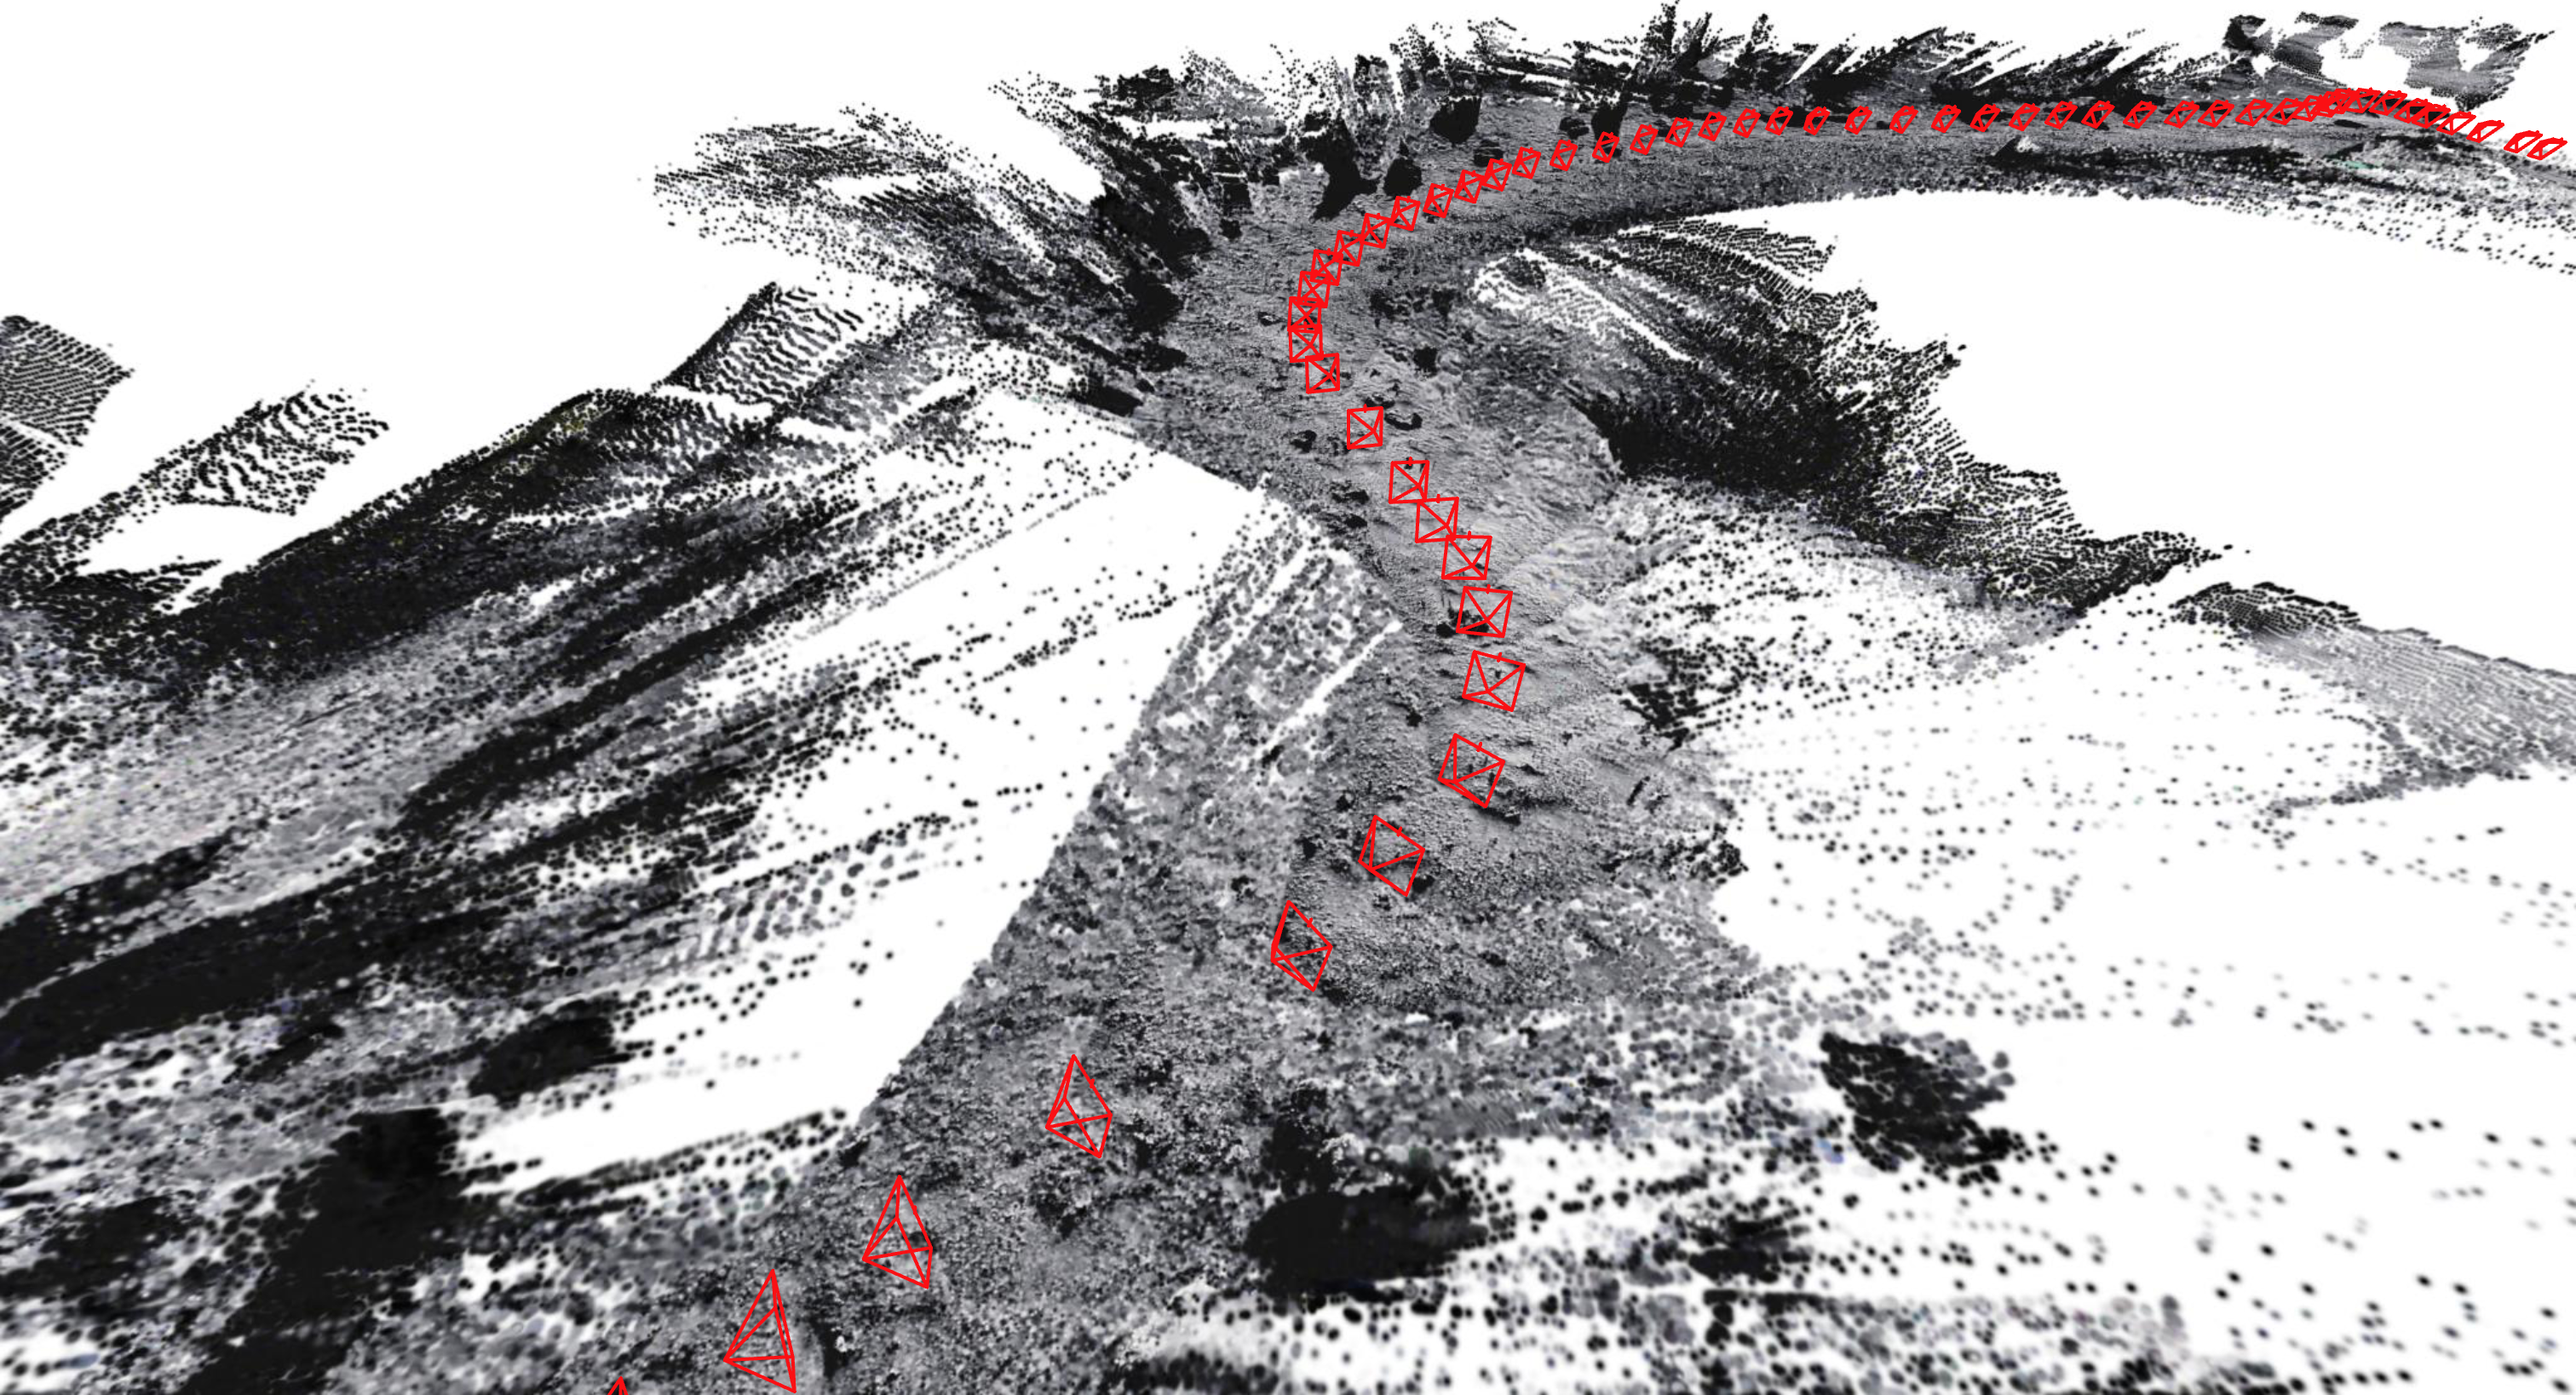
\includegraphics[width=\linewidth]{figures/3dgs/render-2.png}
	\end{subfigure}
	\vspace{1em}
	\begin{subfigure}[b]{0.48\linewidth}
		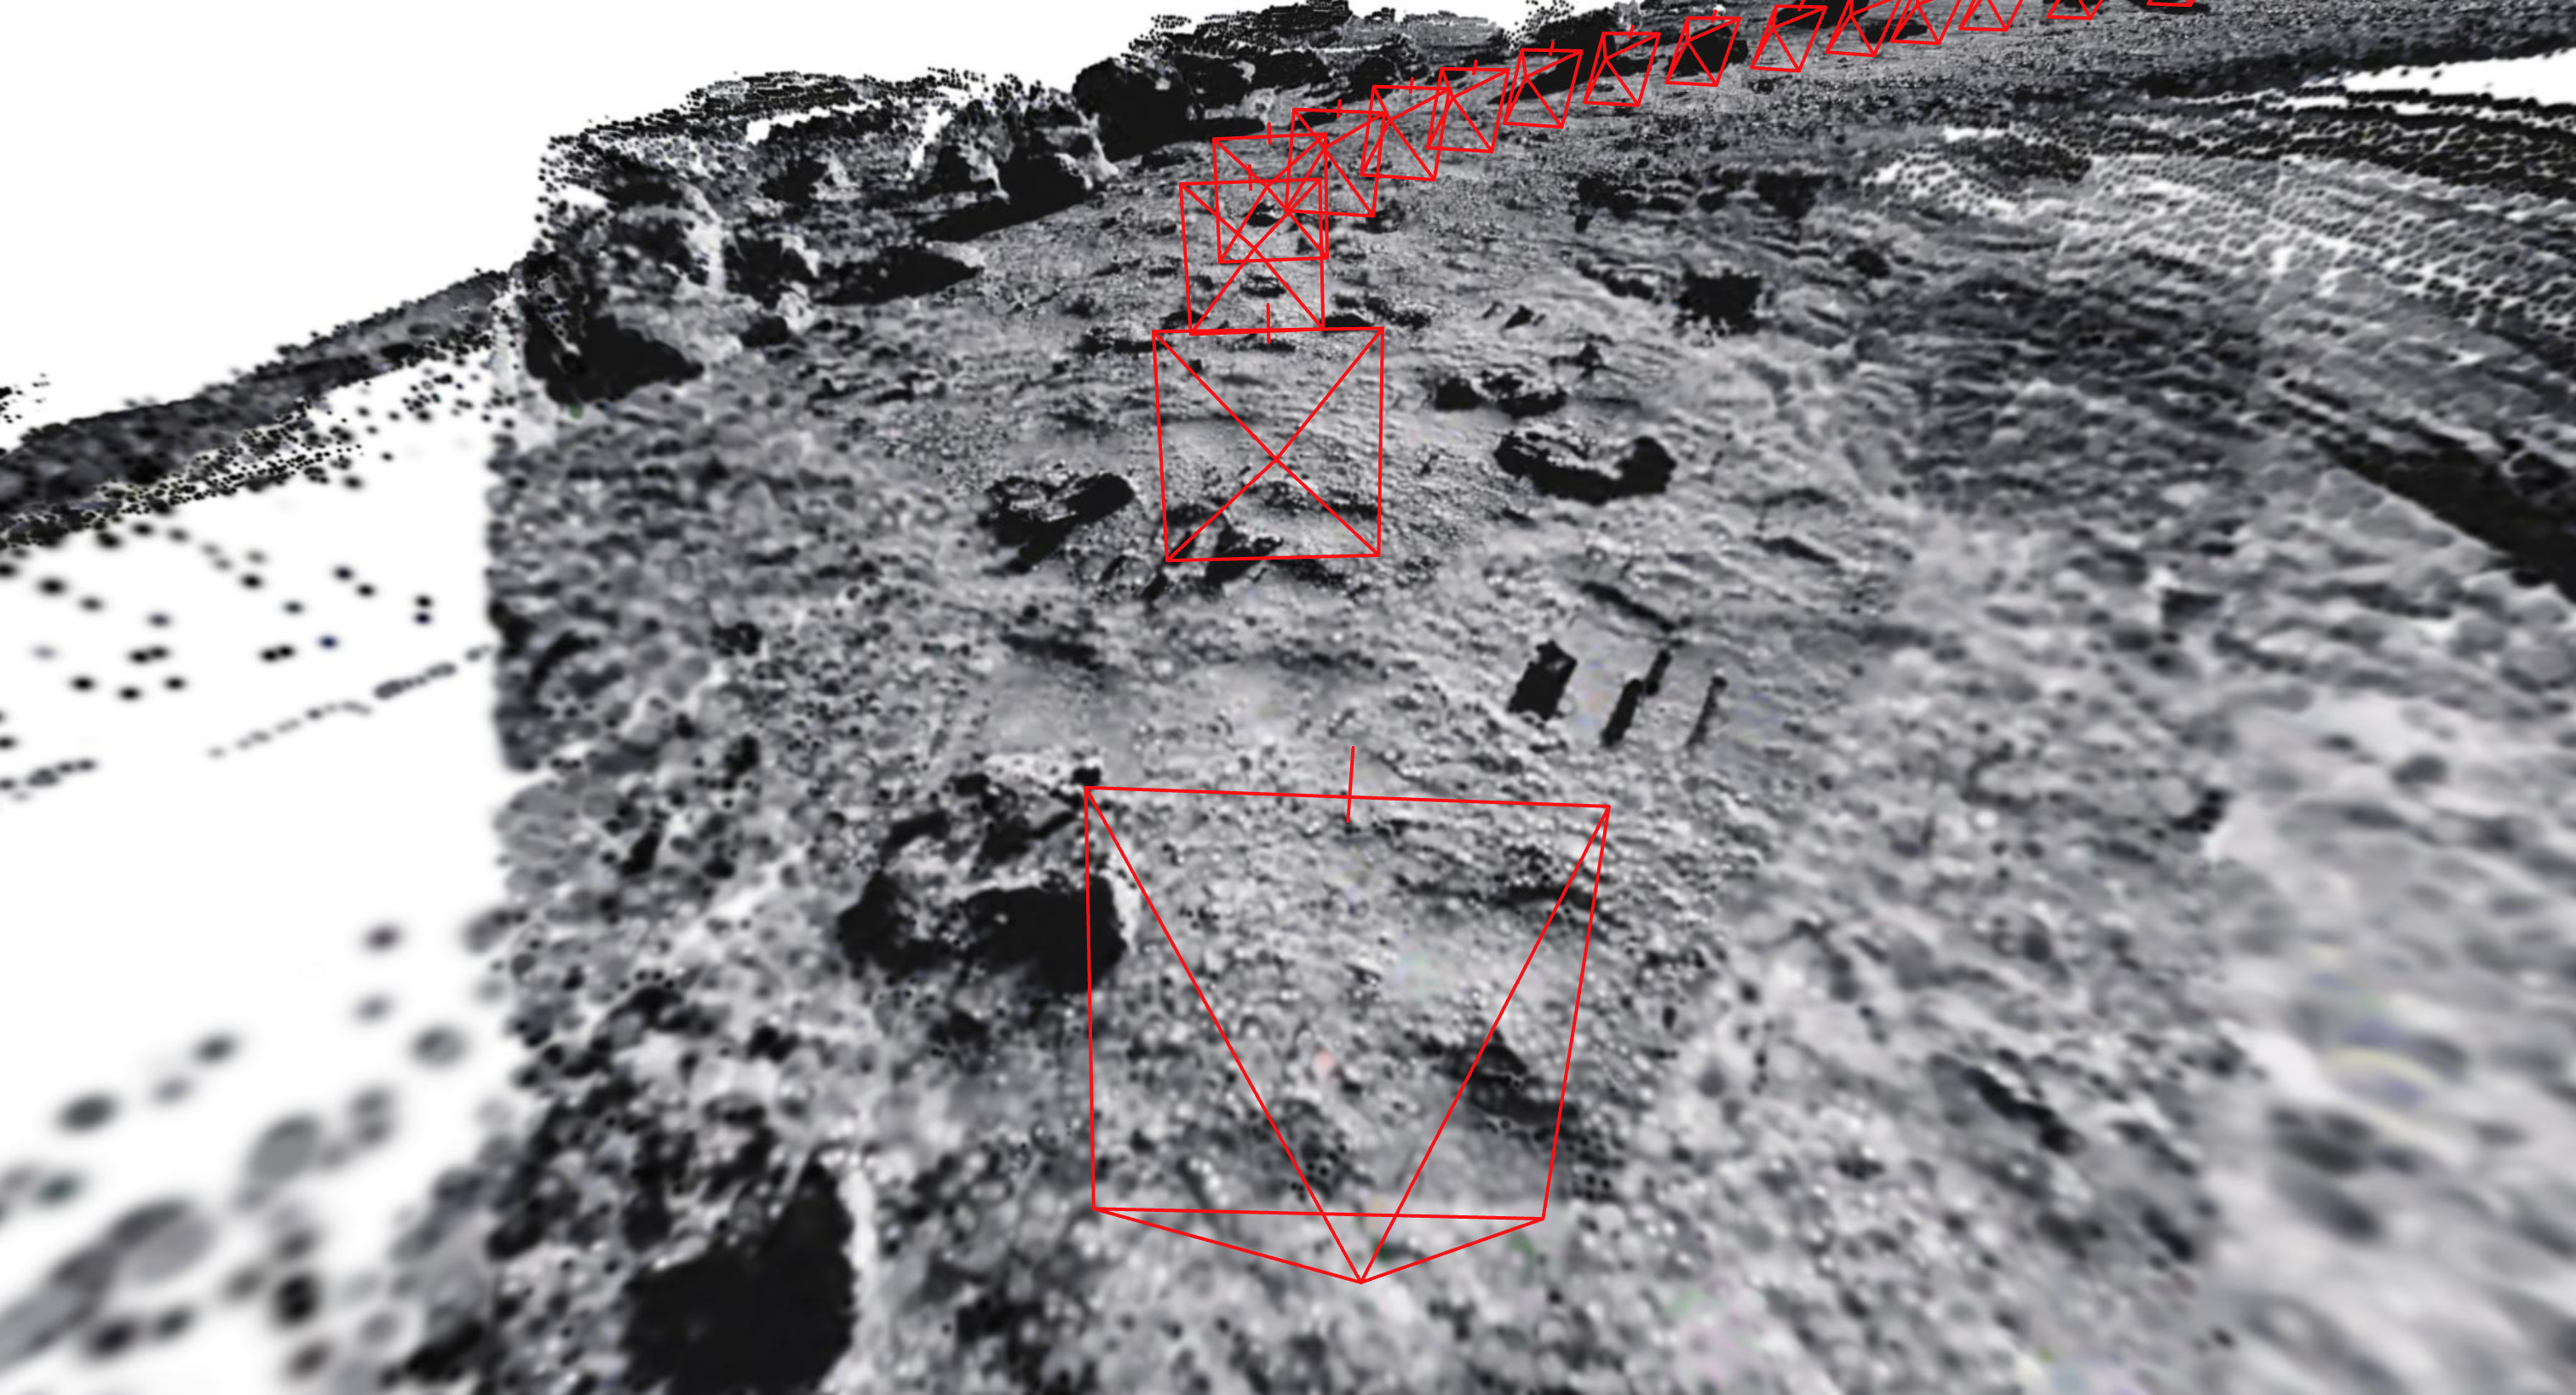
\includegraphics[width=\linewidth]{figures/3dgs/render-3.png}
	\end{subfigure}
	\hfill
	\begin{subfigure}[b]{0.48\linewidth}
		\includegraphics[width=\linewidth]{figures/3dgs/render-4.png}
	\end{subfigure}
	\caption{\bfseries Qualitative results of the real-time 3DGS reconstruction.}
	\label{fig:surface_recon_qual}
\end{figure*}

We implemented our own real-time 3DGS reconstruction pipeline based on Splat-SLAM~\cite{sandstrom_splat-slam_2024} and a point cloud mapping baseline. Our implementation uses ground truth pose information and prior terrain knowledge (without rocks or craters) to initialize the scene. For each new image, we use ground truth segmentation to remove sky regions and tag Gaussians with semantic information, compute depth using our depth estimation models, add new Gaussians to the scene based on RGB and depth information (computing their scale), and optimize the scene in the background using past images. The optimization objective includes L1 RGB and depth losses, penalties for Gaussian density above the surface, Structural Similarity Index Measure (SSIM) loss to ensure the reconstructed images maintain proper structural relationships and perceptual quality compared to the input images, and additional Gaussian regularization terms.
Currently, we do not implement splitting and merging of Gaussians, but we remove Gaussians that are far from the prior terrain.
\Cref{fig:splat-slam} shows the steps of the pipeline using the custom Open3D environment.

\Cref{fig:map_3dgs} shows the 3DGS and point cloud map reconstructions on the Open3D environment, Table~\ref{tab:surface_reconstruction} shows the surface reconstruction and rock detection results, and \cref{fig:novel_views} shows a top view of the 3DGS map. Gaussian splatting with RAFT-Stereo depth outperforms the point cloud baseline in reconstruction accuracy, likely due to its joint optimization over depth and RGB data across multiple views. This demonstrates the potential of neural scene representations for SLAM applications. When ground truth depth is used, the point cloud baseline performs slightly better. We attribute this to our current approach of reconstructing the mesh from the centers of the Gaussians rather than accounting for their density.

In both cases, most errors occur around rocks, which are often dark and hard to distinguish from the sky, making depth estimation challenging. Rock detection performance is comparable between methods, while the point cloud baseline yields lower height error—-possibly due to differences in how the mesh is extracted from the 3DGS map.

\begin{table*}[h]
	\centering
	\small
	\caption{\bfseries Surface reconstruction results. TO BE UPDATED}
	\label{tab:surface_reconstruction}
	\begin{tabular}[t]{|lrrrrrr|}
		\hline
		\multirow{2}{*}{\textbf{Metric}}               &
		\multicolumn{1}{c}{\textbf{Accuracy}}          &
		\multicolumn{1}{c}{\textbf{Completion}}        &
		\multicolumn{1}{c}{\textbf{Precision}}         &
		\multicolumn{1}{c}{\textbf{Recall}}            &
		\multicolumn{1}{c}{\textbf{F-Score}}           &
		\multicolumn{1}{c|}{\textbf{Height Error}}
		\\
		\multicolumn{1}{|c}{}                          &
		\multicolumn{1}{c}{\textbf{[cm] $\downarrow$}} &
		\multicolumn{1}{c}{\textbf{[cm] $\downarrow$}} &
		\multicolumn{1}{c}{\textbf{[\%] $\uparrow$}}   &
		\multicolumn{1}{c}{\textbf{[\%] $\uparrow$}}   &
		\multicolumn{1}{c}{\textbf{[\%] $\uparrow$}}   &
		\multicolumn{1}{c|}{\textbf{[cm] $\downarrow$}}
		\\
		\hline\hline
		\multicolumn{7}{|l|}{\textbf{3DGS}}                                                       \\
		Rock                                           & 61.3  & 27.0 & 13.7 & 26.7 & 18.1 & 15.4 \\
		Regolith                                       & 12.9  & 28.0 & 60.0 & 66.8 & 63.2 & 8.2  \\
		Crater                                         & 941.1 & 27.0 & 9.9  & 15.3 & 12.0 & 74.6 \\
		All                                            & 17.5  & 25.8 & 53.2 & 60.7 & 56.7 & 10.4 \\
		\multicolumn{7}{|l|}{\textbf{ + Ground Truth Depth and Segmentation}}                     \\
		Rock                                           & 61.3  & 27.0 & 13.7 & 26.7 & 18.1 & 15.4 \\
		Regolith                                       & 12.9  & 28.0 & 60.0 & 66.8 & 63.2 & 8.2  \\
		Crater                                         & 941.1 & 27.0 & 9.9  & 15.3 & 12.0 & 74.6 \\
		All                                            & 17.5  & 25.8 & 53.2 & 60.7 & 56.7 & 10.4 \\
		\hline
		\multicolumn{7}{|l|}{\textbf{Point Cloud}}                                                \\
		Rock                                           & 61.3  & 27.0 & 13.7 & 26.7 & 18.1 & 15.4 \\
		Regolith                                       & 12.9  & 28.0 & 60.0 & 66.8 & 63.2 & 8.2  \\
		Crater                                         & 941.1 & 27.0 & 9.9  & 15.3 & 12.0 & 74.6 \\
		All                                            & 17.5  & 25.8 & 53.2 & 60.7 & 56.7 & 10.4 \\
		\multicolumn{7}{|l|}{\textbf{+ Ground Truth Depth and Segmentation}}                      \\
		Rock                                           & 61.3  & 27.0 & 13.7 & 26.7 & 18.1 & 15.4 \\
		Regolith                                       & 12.9  & 28.0 & 60.0 & 66.8 & 63.2 & 8.2  \\
		Crater                                         & 941.1 & 27.0 & 9.9  & 15.3 & 12.0 & 74.6 \\
		All                                            & 17.5  & 25.8 & 53.2 & 60.7 & 56.7 & 10.4 \\
		\hline
	\end{tabular}
\end{table*}



\begin{table}[h]
	\centering
	\small
	\caption{\bfseries Memory usage for 3DGS.}
	\label{tab:memory_usage}
	\begin{minipage}[t]{0.48\linewidth}
		\centering
		\begin{tabular}[t]{|lr|}
			\hline
			\textbf{GPU VRAM} & 1017 MB \\\hline\hline
			\textbf{3DGS}     & 793 MB  \\
			~~Means           & 170 MB  \\
			~~Scales          & 170 MB  \\
			~~Rotations       & 227 MB  \\
			~~Opacities       & 56 MB   \\\hline
			\textbf{Strategy} & 224 MB  \\
			~~Radii           & 56 MB   \\
			~~Labels          & 56 MB   \\
			~~Gradients       & 56 MB   \\
			~~Counts          & 56 MB   \\\hline
		\end{tabular}
	\end{minipage}%
	\begin{minipage}[t]{0.48\linewidth}
		\centering
		\begin{tabular}[t]{|lr|}
			\hline
			\textbf{System RAM} & 1900 MB \\\hline\hline
			~~RGBs              & 1200 MB \\
			~~Depths            & 400 MB  \\
			~~Masks             & 200 MB  \\
			~~Labels            & 100 MB  \\
			\hline
		\end{tabular}
	\end{minipage}
\end{table}

\section{Conclusions}
\label{sec:conclusion}
In this work, we presented and evaluated a real-time framework for creating dense, semantic 3D maps of the lunar surface. Our approach integrates dense perception networks with a 3D Gaussian Splatting (3DGS) representation to address the unique challenges of lunar environments. The primary contributions are the benchmarking of modern perception models for this domain and the demonstration of their integration into an incremental, high-fidelity mapping pipeline.

Our experimental evaluation on the LuSNAR dataset provided several key findings. We identified RAFT-Stereo as a suitable depth estimation model, offering a robust balance between accuracy and real-time processing speed. For semantic segmentation, U-Net++ was selected for its superior performance in detecting rocks, a critical capability for hazard avoidance; its effectiveness was confirmed by the fact that using ground truth segmentation provided no quantitative improvement to the final map. When using these models, our pipeline achieved a geometric height accuracy of approximately 10 cm. Under the assumption of perfect poses, the reconstruction quality was comparable to a traditional point cloud baseline, with the largest errors occurring in distant, poorly-lit craters and along the dark edges of rocks where perception models are most likely to fail.

This work establishes a foundation for several avenues of future research. The most critical next step is to integrate a tracking front-end to create a complete Simultaneous Localization and Mapping (SLAM) system. This will remove the reliance on ground truth poses and test the 3DGS representation's ability to jointly refine the map and camera trajectory, which we hypothesize will show a significant advantage over simpler aggregation methods. Future work will also focus on more sophisticated, density-based techniques for surface extraction from the Gaussians to better capture the continuous geometry. Finally, a more rigorous characterization of the system—including its performance with varied camera configurations, additional datasets, and the incorporation of perception uncertainty—is necessary to develop advanced, map-aware path planning algorithms that can directly enhance rover autonomy.
\section*{Acknowledgements}
% Per the guidelines from the IEEE, any use of AI in the writing
% or preparation (figures, charts, tables, etc.) of a manuscript
% should be disclosed in the Acknowledgements section of the
% paper. Detailed information on the guidelines can be found
% at the IEEE website below. General guidance is that authors
% should acknowledge any use of AI, along with the system
% used, specific sections of the manuscript that are affected, and
% an explanation of the level at which the AI system was used
% to generate content.

We gratefully acknowledge Blue Origin for funding this project and for valuable discussions that contributed to its development.
This manuscript benefited from the use of AI-based assistants, including Claude Sonnet 4.5 and Gemini 2.5 Pro, which were employed for coding assistance and revising. All final content was reviewed and edited by the authors.


\small
\bibliographystyle{IEEEtran}
\bibliography{refs}


\thebiography

\begin{biographywithpic}
{Guillem Casadesus Vila}{figures/bio/Guillem_Casadesus_Vila_Photo.jpg}
is a Ph.D. candidate in the Department of Aeronautics and Astronautics at Stanford University. He received his B.Sc. degree in Aerospace and Telecommunications Engineering in 2022 from the Universitat Politecnica de Catalunya (UPC) under the CFIS program. His research interests include robotic space exploration and space navigation and communication.
\end{biographywithpic} 

\begin{biographywithpic}
{Adam Dai}{figures/bio/adam_dai_profile_ieee.jpg}
is a Ph.D. candidate in the Department of Electrical Engineering at Stanford University. He received his B.Sc. degree in Electrical Engineering with a minor in Computer Science in 2019 from the California Institute of Technology. His research interests include navigation, mapping, and planning in unstructured 3D environments.
\end{biographywithpic} 

\begin{biographywithpic}
{Grace Gao}{figures/bio/gracegao_profilephoto.jpg}
is an assistant professor in the Department of Aeronautics and Astronautics at Stanford University.
Before joining Stanford University, she was an assistant professor at University of Illinois at Urbana-Champaign.
She obtained her Ph.D. degree at Stanford University.
Her research is on robust and secure positioning, navigation, and timing with applications to manned and unmanned aerial vehicles, autonomous driving cars, as well as space robotics.
\end{biographywithpic}
\vfill

\end{document}
